\documentclass[20pt,margin=1in,innermargin=-4.5in,blockverticalspace=-0.25in]{tikzposter}
\geometry{paperwidth=33.11in,paperheight=46.81in} %A0
% \geometry{paperheight=33.11in,paperwidth=23.4in} %A1
\usepackage[utf8]{inputenc}
\usepackage{amsmath}
\usepackage{amsfonts}
\usepackage{amsthm}
\usepackage{amssymb}
\usepackage{mathrsfs}
\usepackage{graphicx}
\usepackage{amsrefs}
\newcommand{\mycomment}[1]{}
\graphicspath{ {images/} }
\usepackage[export]{adjustbox}
\usepackage{enumitem}
%\usepackage[backend=biber, style=numeric]{biblatex}
\usepackage{ubtheme}
\makeatletter
\setlength{\TP@visibletextwidth}{31.0in}
\setlength{ \TP@visibletextheight}{45in}
\makeatother
\usepackage{mwe} % for placeholder images
\usepackage{bm}
\usepackage{bbm}
\definecolor{bristolred}{HTML}{B01C2E}
%\addbibresource{refs.bib}

% set theme parameters
\tikzposterlatexaffectionproofoff
\usetheme{UBTheme}
\usecolorstyle{UBStyle}
\usepackage{comment}
%\usepackage{ragged2e}
\usepackage{mathtools}
%\usepackage[numbers]{natbib}
\usepackage{amsmath,amssymb,amsthm,mathrsfs}
%\usepackage{xfrac}
\usepackage{xcolor}
\usepackage{amsfonts}
\usepackage{tikz}
\usepackage{tikz-3dplot}
\usepackage{pgfplots}
\pgfplotsset{compat=newest}
\usetikzlibrary{decorations.markings}
%\usepackage{graphicx}
%\usepackage[english]{babel}
%\usepackage[utf8x]{inputenc}
\usepackage[scaled]{helvet}
\renewcommand\familydefault{\sfdefault} 
\renewcommand{\vec}[1]{\bm{#1}}
\newcommand{\Tr}{\text{Tr}}
\usepackage[T1]{fontenc}
\newcommand{\qrfac}[2]{{\left({#1}\right)_{#2}}} % suppressing q
\newcommand{\pqrfac}[3]{{\left({#1};#3\right)_{#2}}}
\newcommand{\prodl}{\prod\limits}


\title{\parbox{0.5\linewidth}{Generalised Stokes Theorem}}
\author{\textbf{Vishnu Varadarajan}}
\institute{Ashoka University}

\titlegraphic{
\includegraphics[width=0.3\textwidth]{ashoka-logo.png} \hspace*{4cm}}

\tikzset{arrmark/.style={postaction={decorate,decoration={markings,
mark=at position #1/11-0.1/11 with {\arrow[orange]{<};},
mark=at position #1/11+0.1/11 with {\arrow[orange]{>};}}}}}

\begin{document}
\maketitle
\centering
    \begin{columns}
        \column{0.5}
        \block{Context}{
            
            \begin{itemize}
                \item Gauss was studying surfaces, and wanted to define curvature in a way that was independent of the $3$-dimensional space that the surface is embedded in. The vector calculus view of surfaces is an extrinsic view. But there is also an intrinsic geometry of these surfaces. This intrinsic view of surfaces is developed in the theory of manifolds.
                \begin{center}
                    \begin{tikzpicture}
                        \draw[<->, thin] (-10,0) to (-5,0) node[above left=10pt] {$\mathbb{R}$};
                        \draw[red, thick] (-9,0) node{$\circ$} to (-6,0) node{$\circ$};

                        \draw[<->, thin] (-4,0) to (1,0) node[above left=10pt] {$\mathbb{R}^2$};
                        \draw[<->, thin] (-1.5,-2.5) to (-1.5, 2.5);
                        \node[red] (A) at (-3,1.5) {$\circ$};
                        \node[red] (B) at (0,-1.5) {$\circ$};
                        \draw[red, bend right] (-3,1.5) to (-1.5,0);
                        \draw[red, bend right] (0,-1.5) to (-1.5,0);
                    \end{tikzpicture} \quad
                    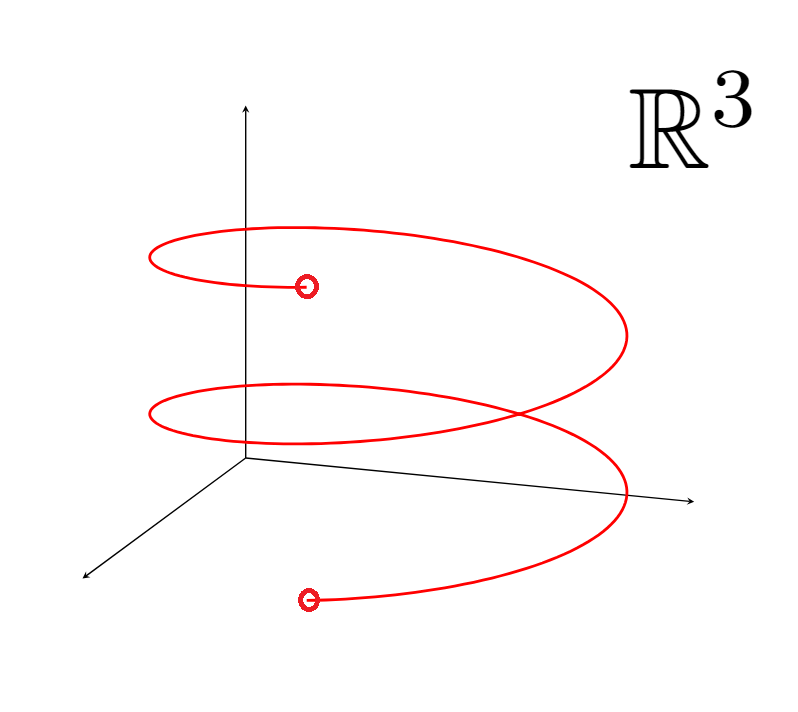
\includegraphics[scale=0.4]{lineinr3.png} 
                    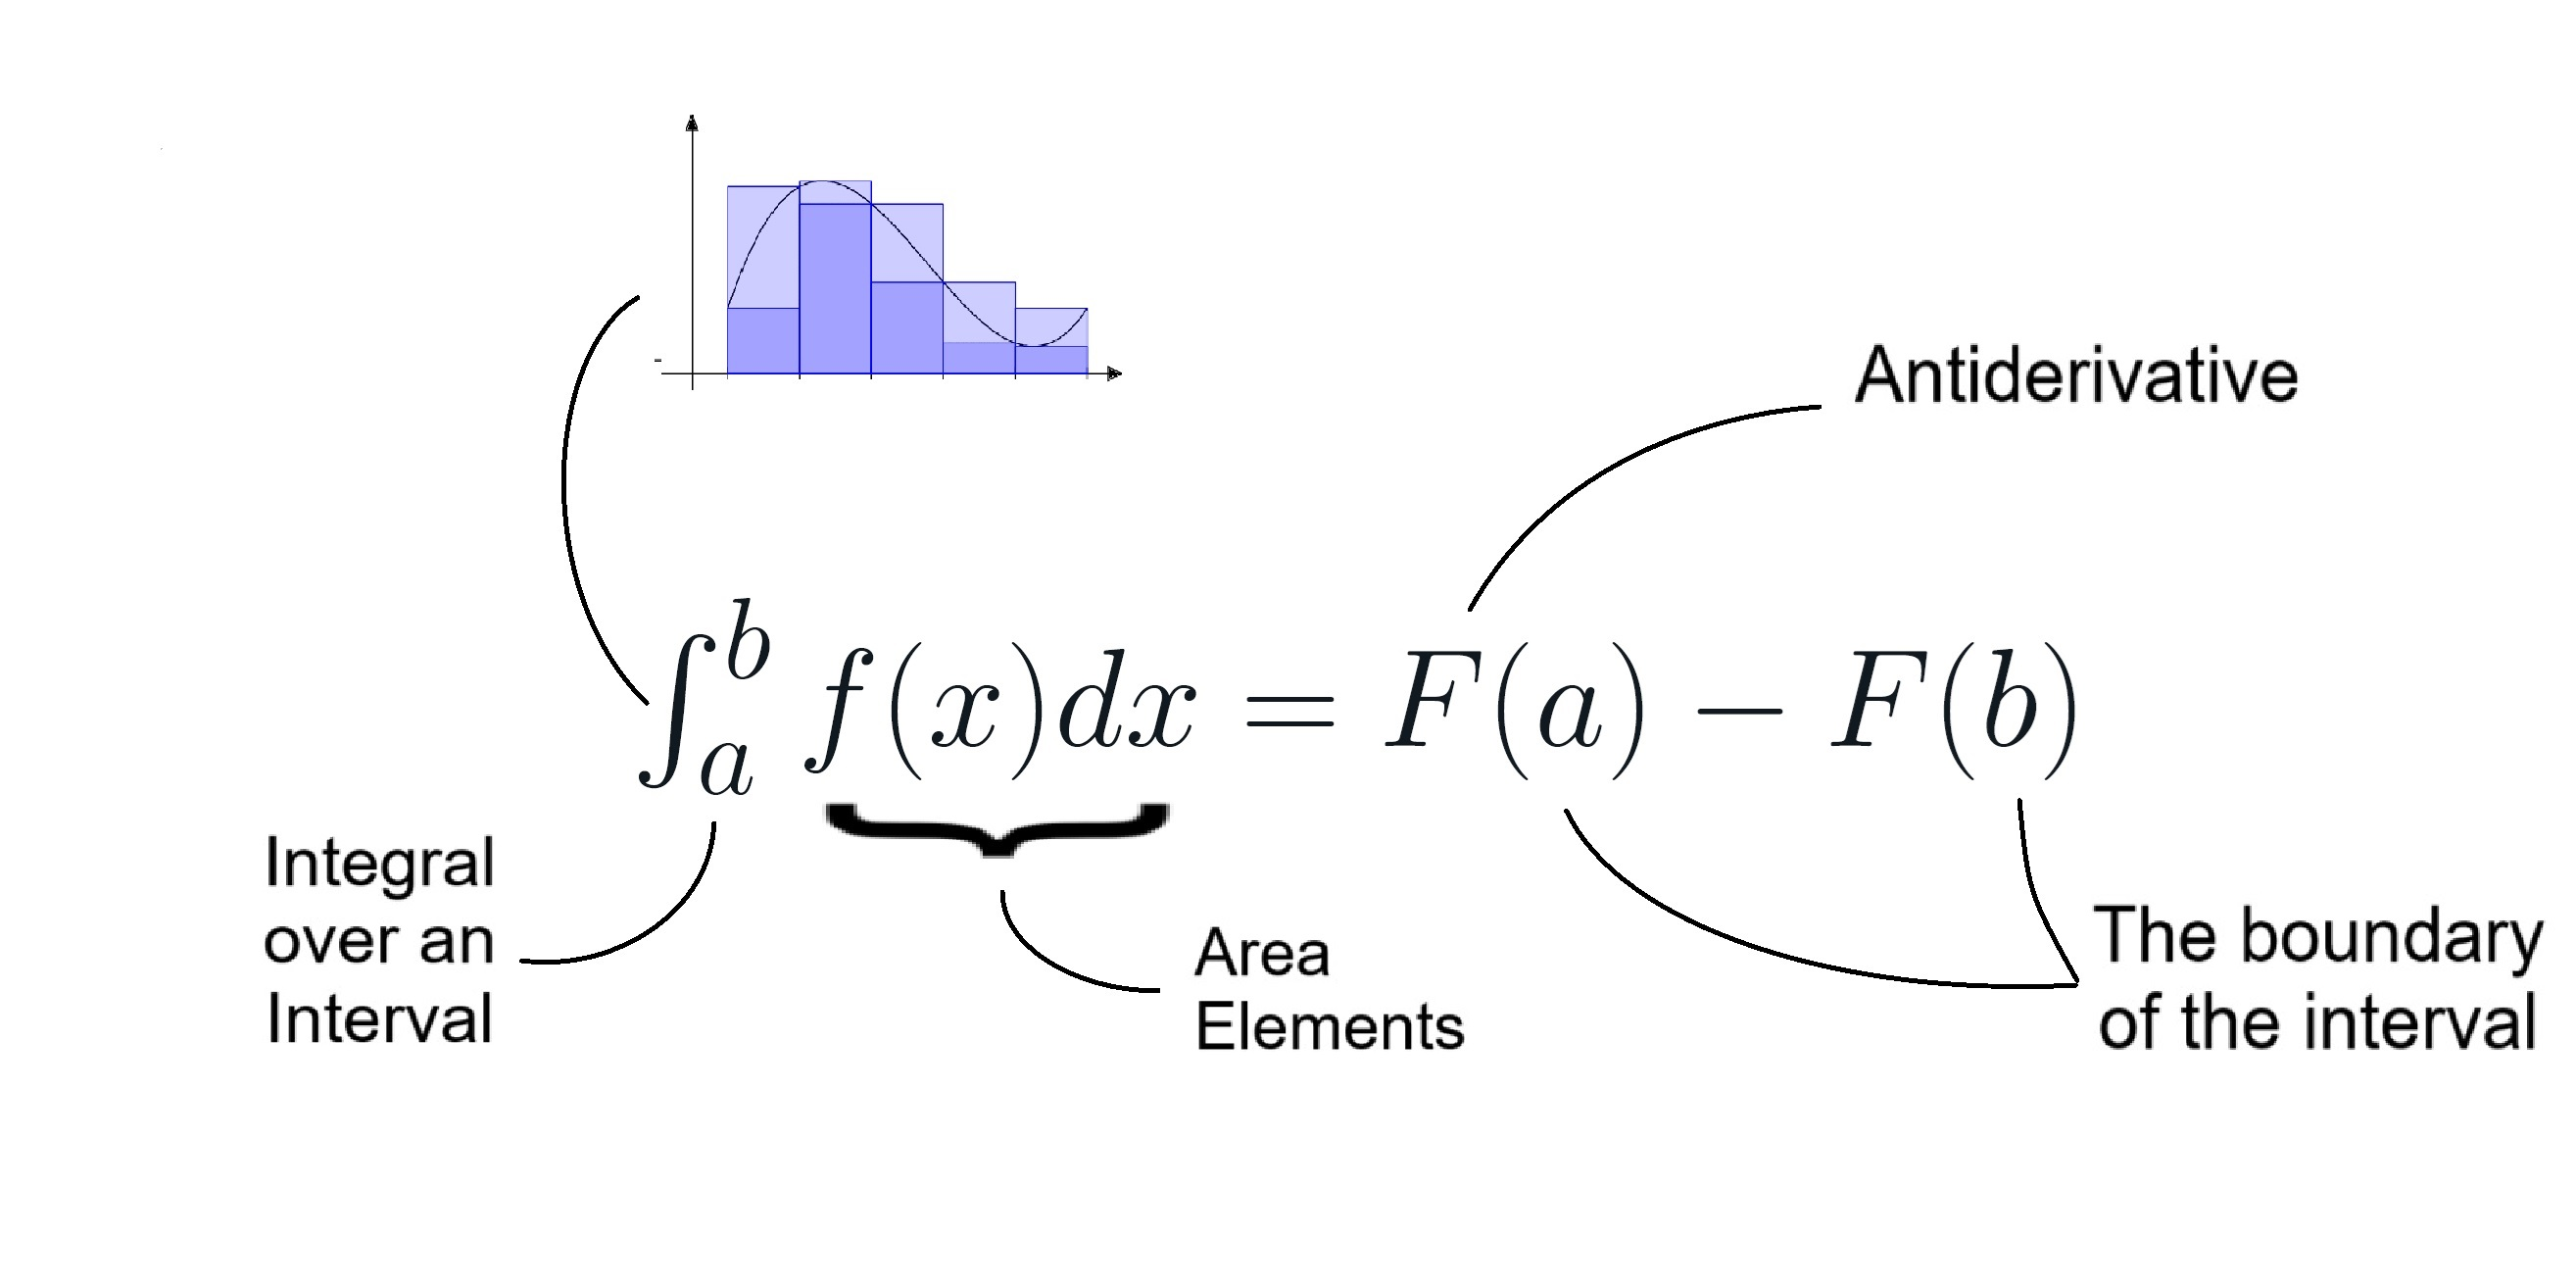
\includegraphics[scale=0.27]{ftc.jpg}
                \end{center}
                
                \item The generalised Stokes theorem is an analog to the fundamental theorem of calculus, in the setting of manifolds
            \end{itemize}
        }
        \block{Manifolds}{
            \begin{itemize}
                \item \textbf{Manifolds} are a topological space such that each point is locally homeomorphic to an open set in an Euclidean space. ($\mathbb{R}^n$). \textbf{Manifolds with boundary} are manifolds, but the co-domain of the homeomorphism is an open set in the Euclidean Half-space ($\mathbb{H}^n$)
                \begin{center}
                    % 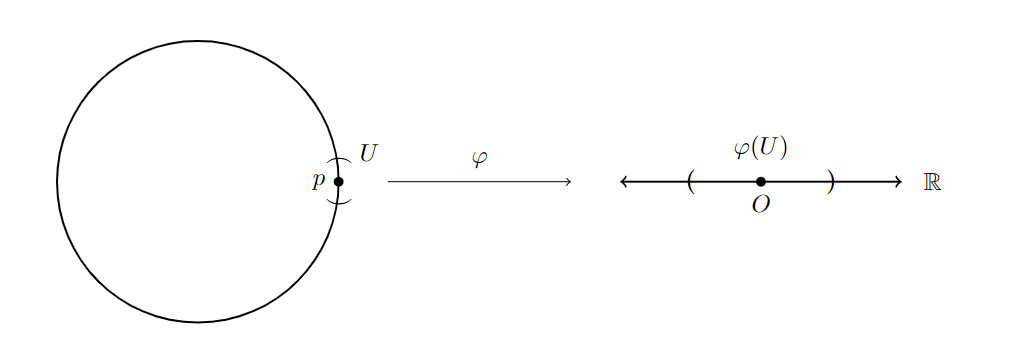
\includegraphics[scale=0.9]{circ1man.png}
                    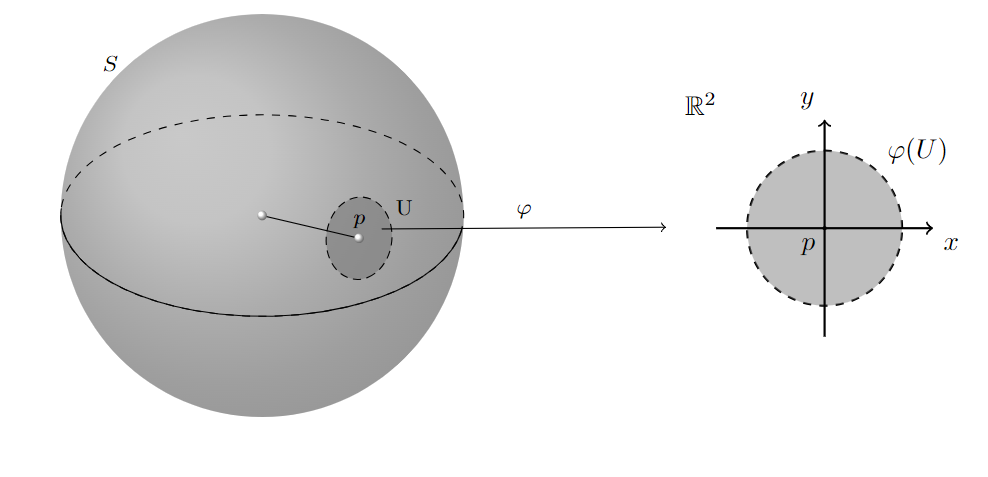
\includegraphics[scale=0.7]{sphere2man.png} \quad \quad \quad \quad \quad \quad
                    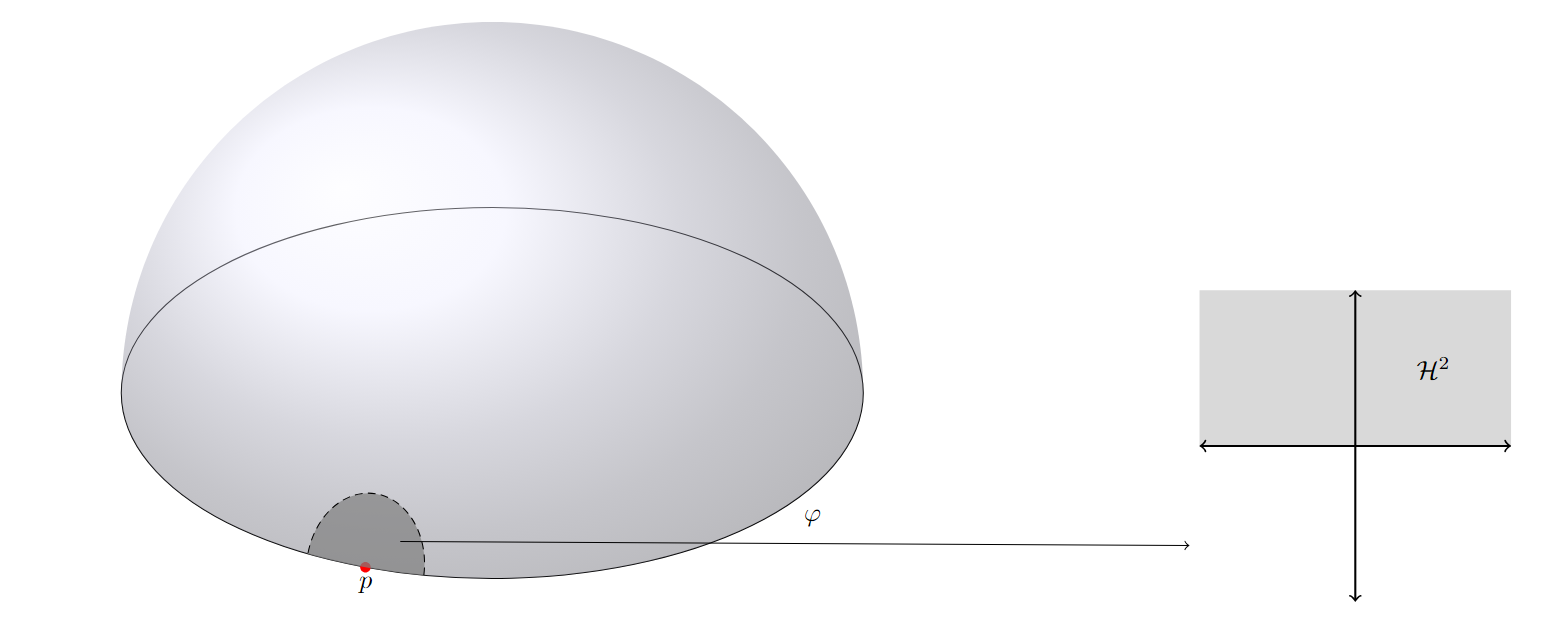
\includegraphics[scale=0.3]{manwbound.png}
                \end{center}
                In the above, the neighborhood paired with the homeomorphism $(U,\varphi)$ is called a \textit{chart}. Because at all points this manifold resembles Euclidean space, a collection of these charts for neighborhoods of each point on the manifold, is given the term \textit{Atlas}.
                \item Tangent Space: Recall the view of tangents as the direction of motion on a path on the surface. We consider paths on the manifold and the directional derivative operator along these paths on functions on the manifold as the tangent vectors. 
                \begin{center}
                    
                        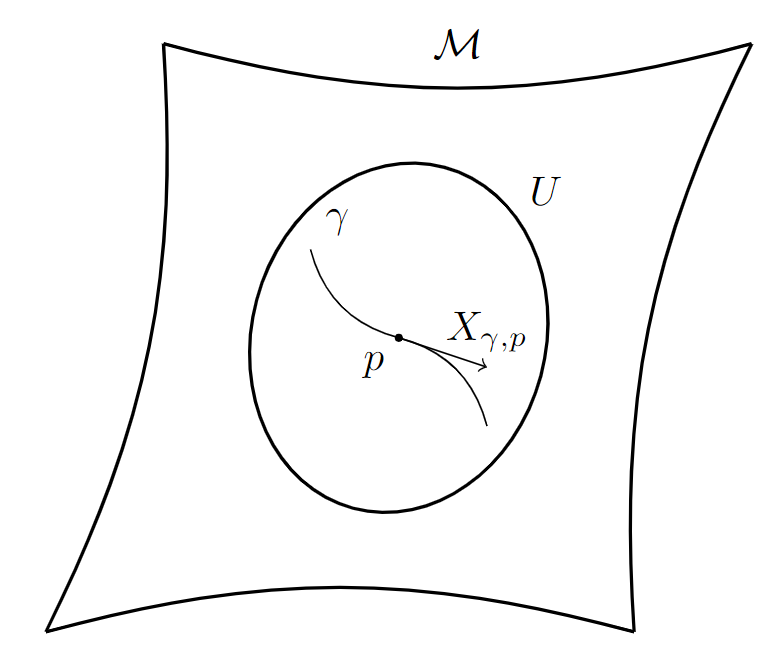
\includegraphics[scale=0.4]{tangentvec.png} 
                        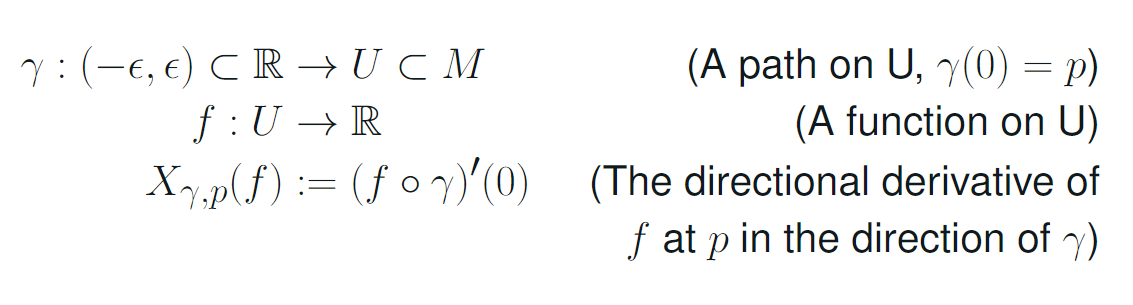
\includegraphics[scale=0.75]{tanvecdetails.png}
                \end{center}
            \end{itemize}
        }
        \block{Differential Forms}{
        \begin{itemize}
            \item The motivation is to figure out what integration on a manifold means. Unlike Euclidean space, smooth manifolds don't have a straightforward way to measure areas when changing coordinates. Integrating a constant function on two spheres of different radii in $\mathbb{R}^3$ gives different results. Both are indistinguishable as $2$-manifolds (diffeomorphic).
            \item Integration over Euclidean surfaces and where that fails on manifolds: infinitesimal area elements. How to measure that on the manifold? Charts don't work as they don't preserve area. 
            \begin{center}
                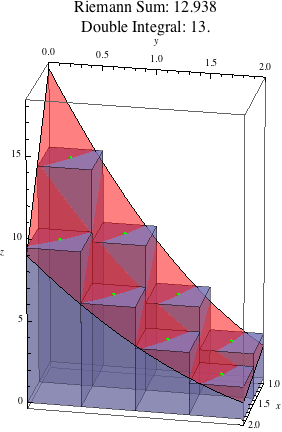
\includegraphics[scale=0.6]{riemannint.png} \quad \quad \quad \quad \quad \quad \quad \quad \quad
                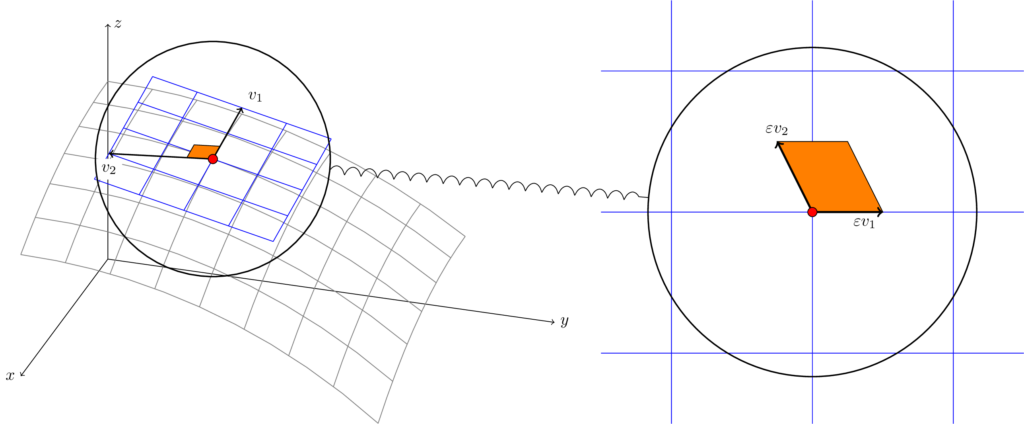
\includegraphics[scale=0.5]{tangentareaelement.png}
            \end{center}
            % \begin{center}
            %     \tdplotsetmaincoords{60}{80}

            %         \begin{tikzpicture}[tdplot_main_coords, scale=7]
            %             % Define axes
            %             \draw[thick,->] (0,0,0) -- (2,0,0) node[anchor=north east]{$x$};
            %             \draw[thick,->] (0,0,0) -- (0,2,0) node[anchor=south east]{$y$};
            %             \draw[thick,->] (0,0,0) -- (0,0,2) node[anchor=south]{$z$};

            %             % Draw the xy-plane
            %             \draw[dashed] (0,0,0) -- (2,2,0);
            %             \draw[dashed] (2,0,0) -- (2,2,0);
            %             \draw[dashed] (0,2,0) -- (2,2,0);

            %             \pgfdeclareverticalshading{custom}{100bp}{
            %                 color(0bp)=(gray!10);
            %                 color(25bp)=(gray!30);
            %                 color(50bp)=(gray!50);
            %                 color(75bp)=(gray!70);
            %                 color(100bp)=(gray!90)
            %             }
                    
            %             % Draw the surface between the curves with custom shading
            %             \path[shading=custom,shading angle=45,opacity=0.7] 
            %                 plot[smooth, tension=0.7] coordinates {(0.1,0.3,0) (1,0.7,0) (0.7,1.2,0) (1.5,1.7,0)}
            %                 -- plot[smooth, tension=0.7] coordinates {(1.5,1.7,1) (0.7,1.2,0.5) (1,0.7,1) (0.1,0.3,1.5)}
            %                 -- cycle;
                    
            %             % Add curved lines to enhance 3D effect and show morphing
            %             \foreach \t in {0,0.2,...,1} {
            %                 \draw[black!50, opacity=0.7] 
            %                     plot[smooth, tension=0.7] coordinates {
            %                         (0.1,0.3,{1.5*\t}) 
            %                         (1,0.7,{\t}) 
            %                         (0.7,1.2,{0.5*\t}) 
            %                         (1.5,1.7,{\t})
            %                     };
            %             }
            %                                 % Draw a smooth path in the xy-plane
            %             \draw[red, thick] plot[smooth, tension=0.7] 
            %                 coordinates {(0.1,0.3,0) (1,0.7,0) (0.7,1.2,0) (1.5,1.7,0) };
            %             \node at (1.5,1.5,0) {$\mathcal{N}$};
            %             \node at (1.5,0.5, 0) {$\mathcal{M} = \mathbb{R}^2$};
            %             \draw[blue, thick] plot[smooth, tension=0.7] 
            %                 coordinates {(0.1,0.3,1.5) (1,0.7,1) (0.7,1.2,0.5) (1.5,1.7,1) };

            %         \end{tikzpicture}
            % \end{center}
            \item At each point on the manifold, we need a way to measure the area of infinitesimal rectangles in a manner independent of coordinates. This is achieved through differential forms. A $k$-form takes an ``infinitesimal $k$-parallelogram'' (edges given by tangent vectors) as input and returns its $k$-volume. When areas come into picture, it is natural to expect multilinearity and antisymmetry. The algebra is developed keeping this in mind. 
            \item Tensors: A $k$-tensor is a multilinear map from $V^k$ to $\mathbb{R}$, where $V$ is a vector space. A tensor is said to be alternating if it changes sign under the interchange of any two of its arguments.
            \[
                T(v_1, \ldots, v_k) = \text{sgn}(\sigma) T(v_{\sigma(1)}, \ldots, v_{\sigma(k)})
            \]
            Tensor Product: combines a $k$-tensor and an $l$-tensor to form a $(k+l)$-tensor. Defined as follows, where $T$ and $S$ are $k$ and $l$ tensors respectively.
            \[
                T \otimes S(v_1, \ldots, v_{k+l}) = T(v_1, \ldots, v_k) S(v_{k+1}, \ldots, v_{k+l})
            \]
            The Alt operator: maps a $k$-tensor to an alternating $k$-tensor.
            \[
                \text{Alt}(T)(v_1, \ldots, v_k) = \frac{1}{k!} \sum_{\sigma \in S_k} \text{sgn}(\sigma) T(v_{\sigma(1)}, \ldots, v_{\sigma(k)}) = \frac{1}{k!} \sum_{\sigma \in S_k} \sigma T \cdot \text{sgn}(\sigma)
            \]
            \item The wedge product: combines $k$-tensor and $l$-tensor to form an alternating $(k+l)$-tensor. It is defined as follows, where $T$ and $S$ are $k$ and $l$ tensors respectively.
            \[
                T \wedge S = \text{Alt}(T \otimes S)
            \]
        \end{itemize}
        A consistent way to measure $k$-volume: a mesh of atoms and counting how many of those lie within the object, multiplied by a scaling factor. Coordinate-independent measurement of area, as any distortion between two charts will imply an equal distortion of the atoms, and the area is conserved.
        }
        

        \column{0.5}
         \block{}{
            
            \begin{center}
                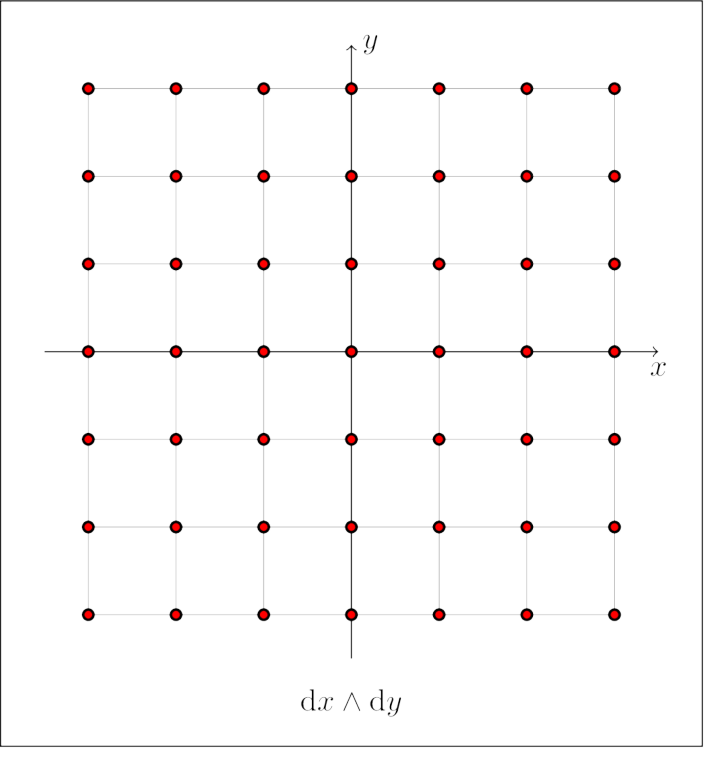
\includegraphics[scale=0.3]{dxdyform.png} \quad
                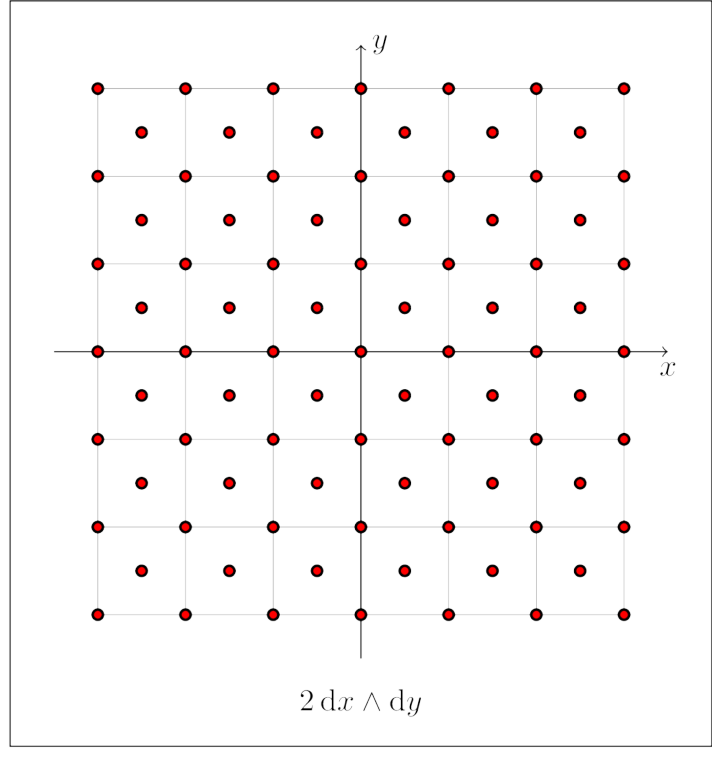
\includegraphics[scale=0.3]{2dxdyform.png} \quad
                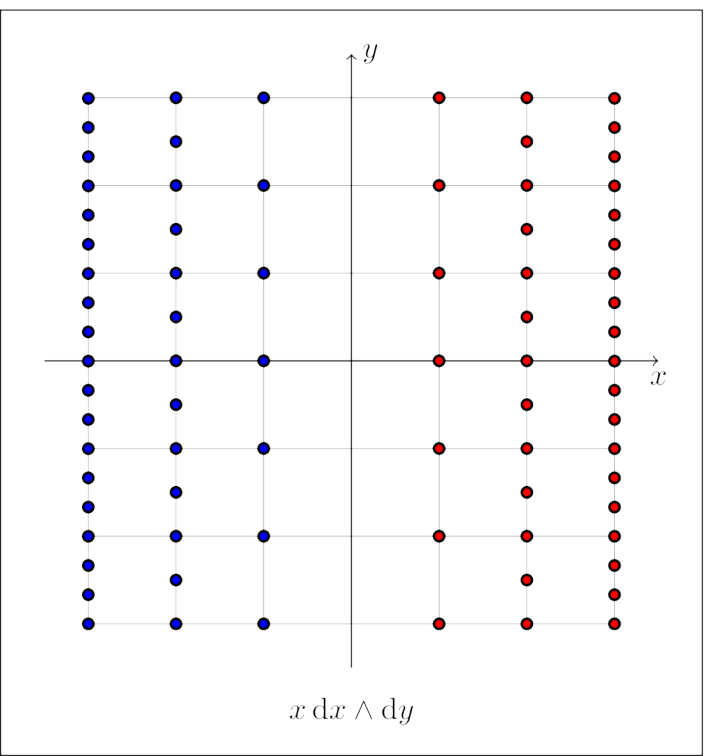
\includegraphics[scale=0.3]{xdxdyform.png} \quad
                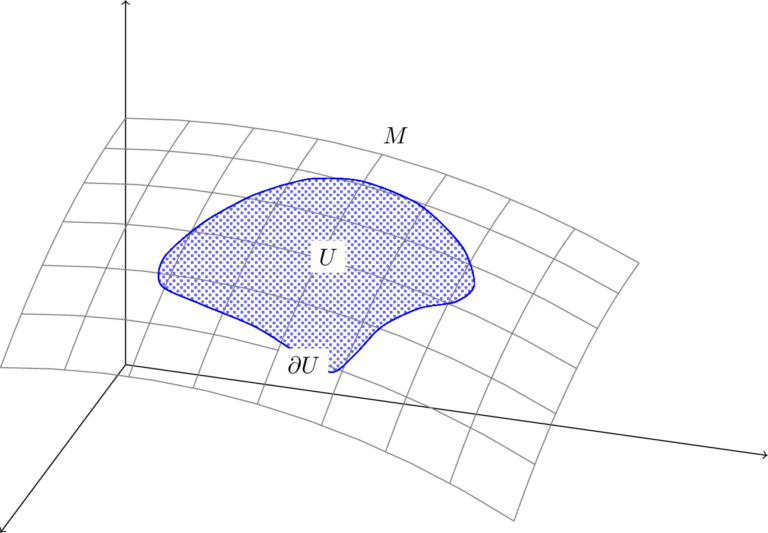
\includegraphics[scale=0.3]{atom-manifolds.png}\quad
                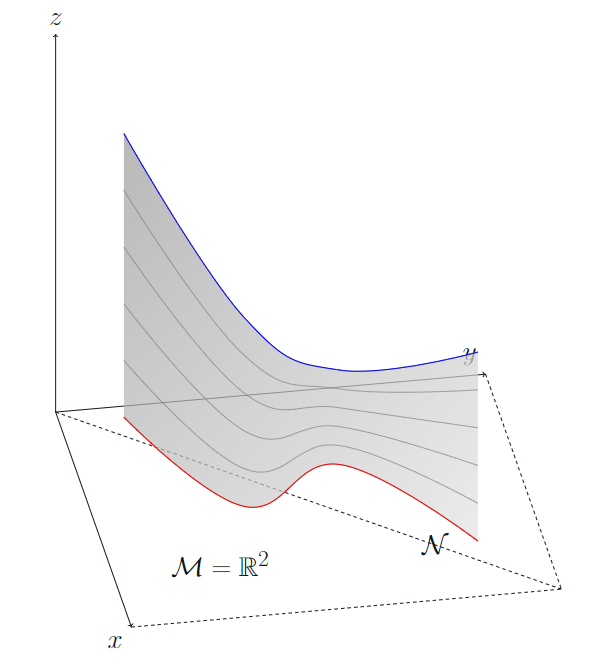
\includegraphics[scale=0.35]{otherformsmotiv.png}
            \end{center}
            With this, we think of a $k$-form as a measuring tape for $k$-dimensional volumes. This motivates an $n$- form on an $n$-manifold but why are other order forms needed? 
            \begin{itemize}
                \item The above definitions are insufficient for integrating over $k$-dimensional subsets (specifically $k$-dimensional submanifolds of $\mathcal{M}$, $\mathcal{N}$) and calculating their $k$-volumes. 
                \item Algebraically, We define a “\( k \)-form on \( \mathcal{M} \)” as an object \( \omega \) that takes \( k \) tangent vectors at the same point of \( \mathcal{M} \), and its restriction to \( \mathcal{N} \) is simply the restriction of \( \omega \) to the collection of vectors tangent to \( \mathcal{N} \).
                \item To visualise it, a $k$-form on $\mathbb{R}^n$ can be seen as a stack of $n-k$ dimensional hyperplanes. The intersection of the hyperplanes and the $k$-dimensional subspace gives points that act as the atoms we use to measure $k$-volume.
                \begin{center}
                    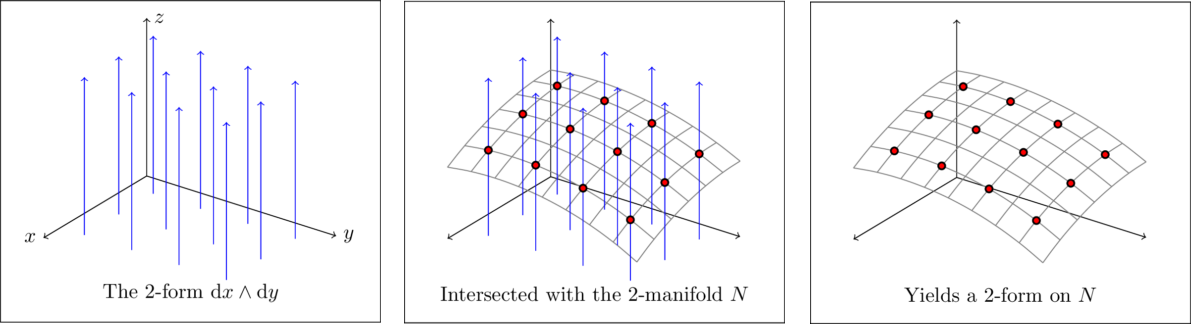
\includegraphics[scale=0.8]{2formsinr3.png} \qquad \qquad
                    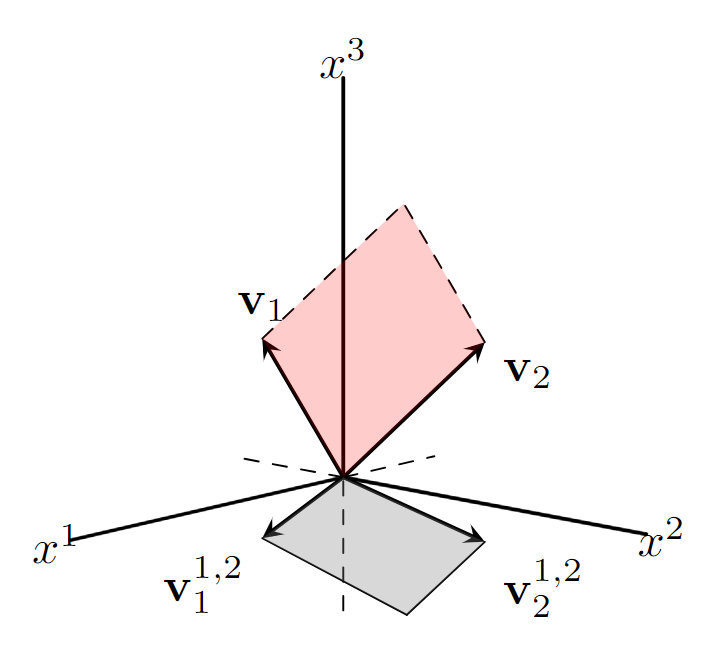
\includegraphics[scale=0.3]{2formasproj.png}
                \end{center}
                \item The basis forms: measuring tapes along the $k$-planes formed by axes.
                \begin{itemize}
                    \item basis $1$-forms: projected lengths, inner product with basis vectors of $\mathbb{R}^n$. $dx_i$.
                    \item basis $k$-forms: $k$-volume of the $k$-parallelogram projected onto the $k$-plane. Wedge products of $k$ basis $1$-forms. $dx_{i_1} \wedge \cdots \wedge dx_{i_k}$.
                \end{itemize}
                \item Extending these to the manifold: at each point, the $k$-form behaves similarly on the tangent space. 
            \end{itemize}
         }
        \block{Exterior Derivative}{
            The exterior derivative of a $k$-form is a $(k+1)$-form.
            \begin{itemize}
                \item If \( f \) is a smooth function (a \( 0 \)-form), then its exterior derivative \( df \) is the differential of \( f \). Specifically, \( df \) is the unique \( 1 \)-form such that for any smooth vector field \( X \),
                \(
                df(X) = d_X f,
                \)
                where \( d_X f \) is the directional derivative of \( f \) in the direction of \( X \). Restricting the form to a chart $U$ with coordinates $x_1, x_2, \cdots x_i$ we get a local expression for the form, \[ df = \sum_i \frac{\partial f}{\partial x_i} dx_i. \]
                \item Given a $k$-form $\omega = \sum_{I} a_I dx^I$, where $I$ is a multi-index, the exterior derivative of $\omega$ is defined as
                \[
                    d\omega = \sum_{I} da_I \wedge dx^I.
                \]

            \end{itemize}
        Consider a form like \( x dy \) in $\mathbb{R}^2$, where the horizontal lines (representing \( dy \)) become more concentrated as you move to the right. As you move to the right from $x=0$, more and more lines are stacked. Same with moving left from $x=0$, but with negative concentration. 

        For a general form, we can think of it as a stack of surfaces. Taking the exterior derivative of a \( k \)-form essentially asks, “What is the boundary of this structure?” 
        \begin{center}
            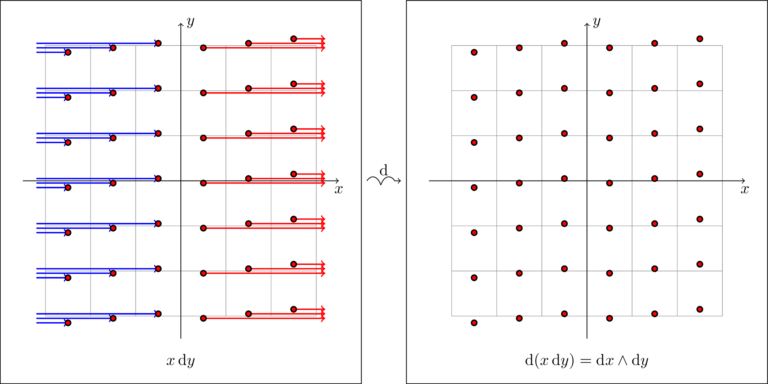
\includegraphics[scale=0.5]{exteriorderivative.png}
            \qquad
            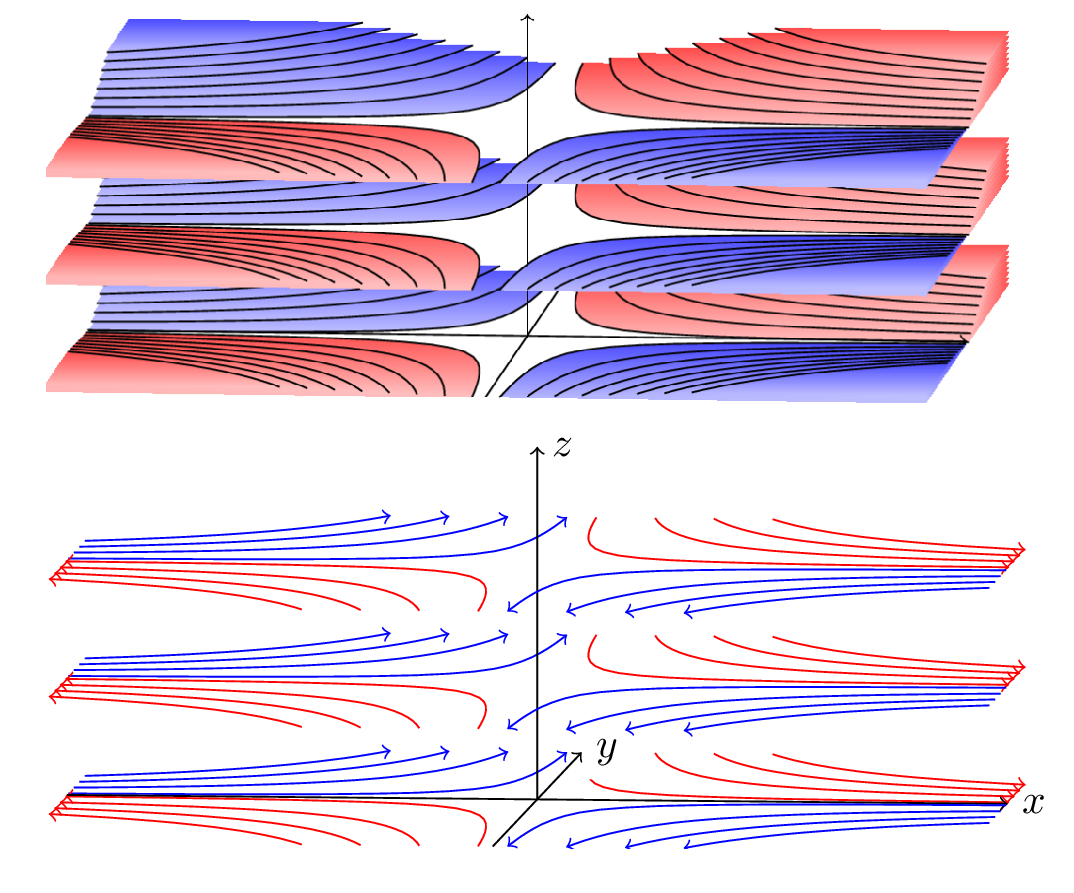
\includegraphics[scale=1]{d of xydz.png}
        \end{center}

        For a form that has no ``boundary", the exterior derivative becomes zero. Or a form like \( x dy \), its boundary becomes a dense collection of points, capturing a notion similar to the familiar \( dx \wedge dy \).
        }
        
        \block{Generalised Stokes Theorem}{
        \begin{itemize}
            \item Consider an \( n \)-dimensional manifold $\mathcal{M}$ with a boundary component $\mathcal{N}$ that separates $\mathcal{M}$ into an ``inside" and ``outside" region. For such a separation to make sense, we require the "inside" to be compact or ``small” enough to avoid infinite extension within $\mathcal{M}$.
            \item Integrating a \( k \)-form \( \omega \) over $\mathcal{N}$, is counting how many field lines enter and exit the boundary. Since $\mathcal{N}$ compactly encloses an interior, any field line that starts inside $\mathcal{N}$ either exits $\mathcal{N}$ or terminates within $\mathcal{M}$. The points where they enter contribute to integration as the positive atoms and those that
        \end{itemize}
            

         If we see integrating an $n-1$-form on $\mathcal{N}$, as counting the planes entering $\mathcal{N}$, we conclude that solving the problem of integrating $\omega$ over $\mathcal{N}$ is the same as to count the number of line ends in $\mathcal{M}$. That is,
         \[
            \int_{\mathcal{\partial M}} \omega = \int_{\mathcal{M}} d\omega.
         \] 

        }
        \block{References}{
                
           }
        
    \end{columns}
\end{document}